\begin{quote}
Participants must bring self-knowledge and no small measure of honesty
to the peer-learning project in order to accurately enunciate their
motivations. If everyone in your peer learning project asks ``What
brings me here?'' ``How can I contribute?'' and ``How can I contribute
more effectively?'' things will really start percolating. Test this
suggestion by asking these questions of yourself and taking action on
the answers!
\end{quote}
The primary motivators reported by participants in the Peeragogy project
include:

\begin{enumerate}
\item
  Acquisition of training or support in a topic or field;
\item
  Building relationships with interesting people;
\item
  Finding professional opportunities through other participants;
\item
  Creating or bolstering a personal network;
\item
  More organized and rational thinking through dialog and debate;
\item
  Feedback about their own performance and understanding of the topic.
\end{enumerate}
Each of those motivators can affect the vitality of the peeragogical
process and the end result for the individual participant.

The various motivations also carry some associated risks. For example,
if one learner's motivation includes a desire to make business contacts,
he or she may be reluctant to share this with the facilitator and other
learners for fear of seeming greedy or commercial. Whether or not
potential peeragogues eventually decide to assume these risks depends on
various factors.

Cultural or societal factors can also complicate motivations and
relationships in the peer-learning environment. Actions that typify
inappropriate behavior in one culture might represent desirable behavior
in another. In the case of culture, motivations can often come out of
the closet through conflict; for example, when one learner feels
offended or embarrassed by the actions of another.

\begin{quote}
\textbf{Philip Spalding}: \emph{``The idea of visiting a garden together
in a group to learn the names of flowers might have been the original
intention for forming a Garden Group. The social aspect of having a day
out might be goal of the people participating.''}
\end{quote}

\begin{center}
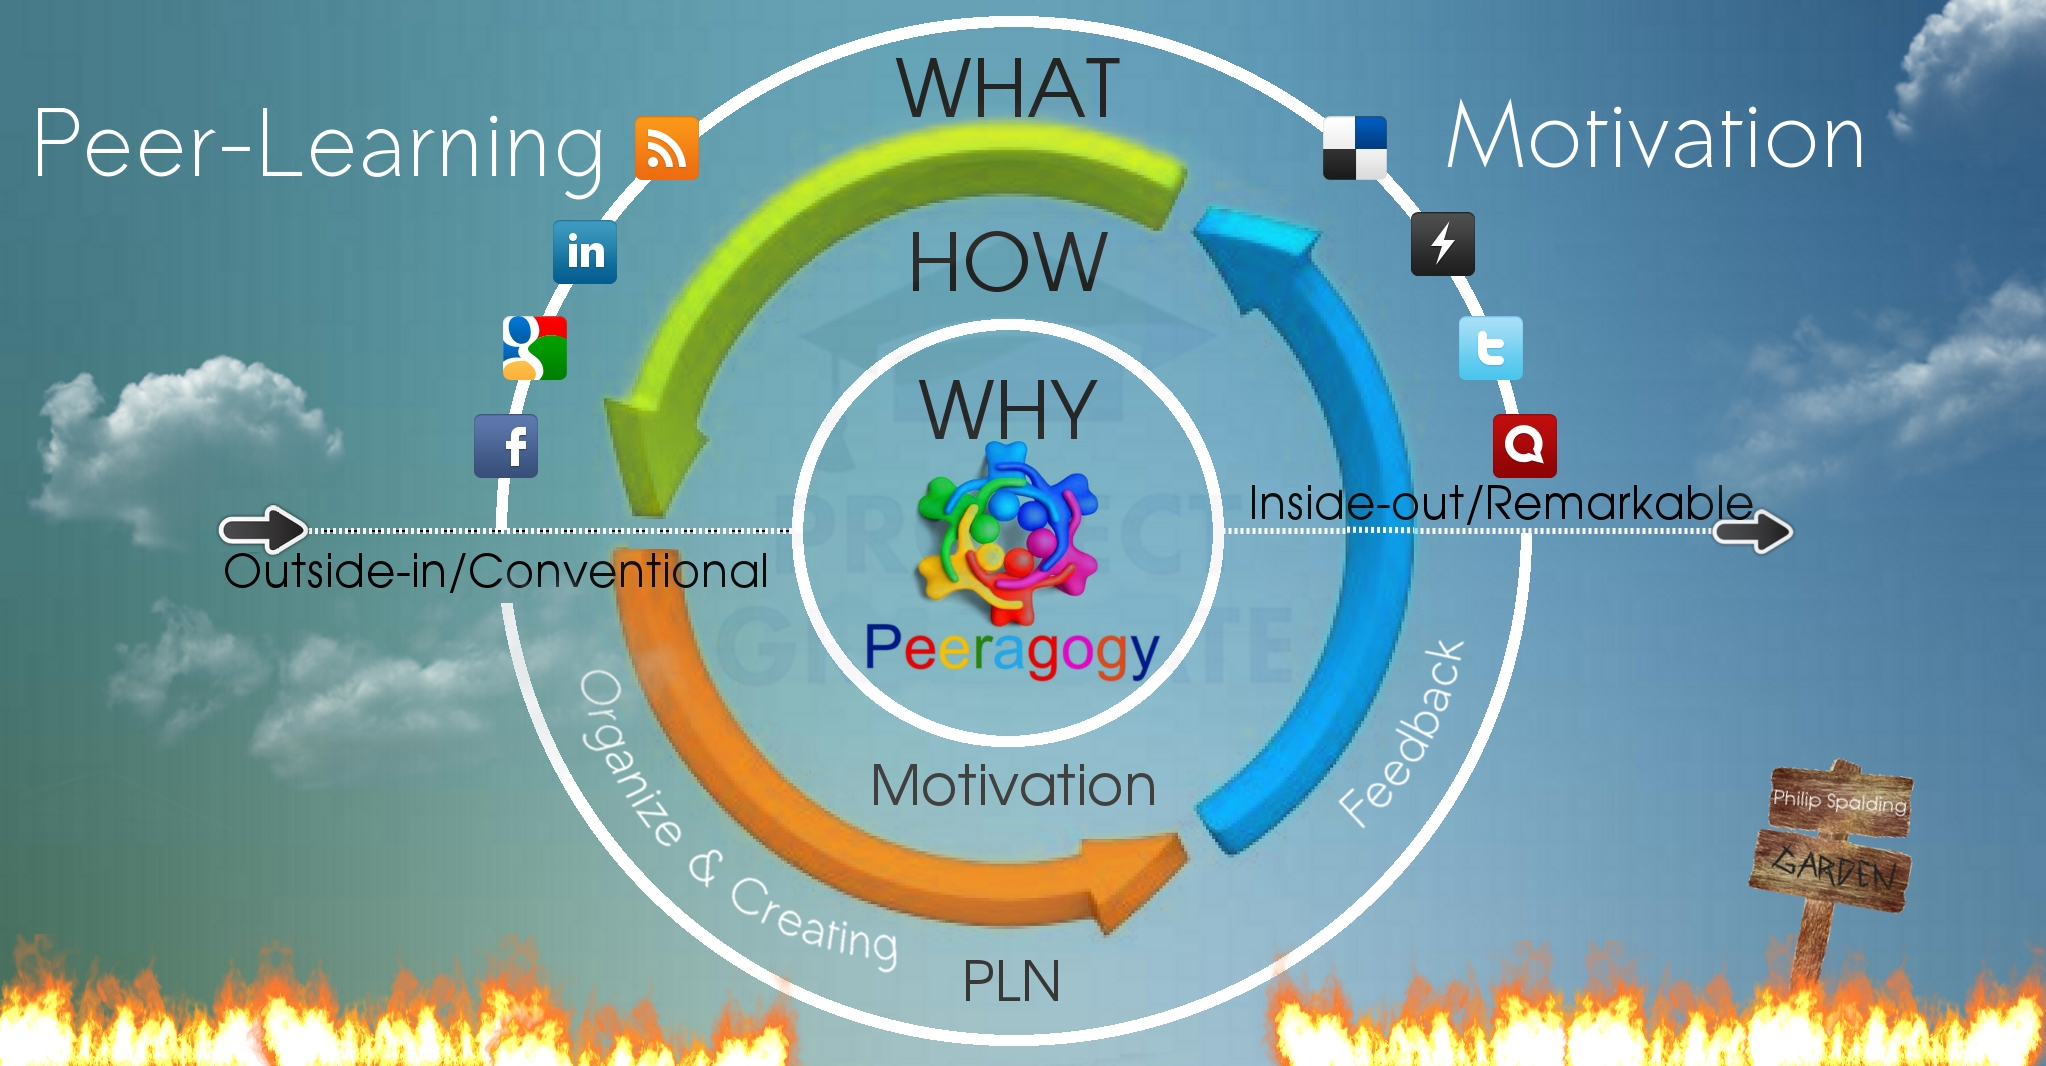
\includegraphics[width=.5\textwidth]{../pictures/pln-cycle.jpg}
\end{center}

\emph{``What's my motivation?''}

\section*{Example: Peeragogy editor Charlotte Pierce}

Basically, I'm here because as an early adopter and admitted gadget
freak, I find it fun and rewarding to explore new technologies and
topics that I feel have a practical or exciting application. But I have
some some other motivations that subtly co-exist alongside my eagerness
to explore and learn.

Howard Rheingold's reputation as an innovator and internet pioneer got
my attention when he announced his Think-Know Tools course on Facebook
in 2012. I had known of Howard from the 1990's when I was a member of
The WELL (Whole Earth `Lectronic Link). I was curious to see what Howard
was up to, so I signed onto the wiki site, paid my \$300, and took the
course starting in October.

Looking back, I realize we were practicing Peeragogy throughout the TKT
course, though at the time I hardly knew peer learning from a pickle. In
late November, missing the camaraderie and challenge of TKT, I stepped
over to check out The Peeragogy Handbook.

Which brings me to motivations in signing on to Peeragogy. Since Howard
and several Think-Know Tools co-learners were already dedicating their
time there and their work looked innovative and exciting, I suspected
they might be onto something that I wanted to be a part of. Plus, my
brain was primed by the TKT experience. ``What if a diverse group of
people could learn a subject with little or no cost and not a lot of
barriers to entry,'' I thought. ``What if their own experience qualified
them to join, contribute, and learn.''

I also thought there might be a chance to meet some potential business
partners or clients there - but if not, the experience looked rewarding
and fun enough for me to take the risk of no direct remuneration. There
was no cost to me, and a wealth of knowledge to gain - and a way to be
part of something new and exciting. These are always big draws for me. I
wanted to be in on it, and nobody was telling me I couldn't!

My projections proved correct. The participants already on board were
gracious in welcoming me to Peeragogy, patient in getting me up to
speed, and persistent in coaxing me into using the tools central to the
project. I connected, learned, grew, and contributed. Now I'm on the
brink of starting a peer learning project of my own in my publishing
organization, IPNE.org. Stay tuned!

\section*{Example: Cafes, schools, workshops}

Suppose we wanted to make Peeragogy into a model that can be used in
schools, libraries, and so forth, worldwide - and, in fact we do! How
can we bring the basic Peeragogy motivations to bear, and make a
resource, plan of action, and process that other people can connect
with? In brief, how do we build peer learning into the curriculum?

\begin{quote}
\textbf{Charlotte Pierce}:\emph{With success, these could possibly raise
awareness while utilizing the existing framework and population of
standard education. A curriculum ``unit'' using peeragogy, for example,
or a seminar in a professional development retreat for teachers. It's
not optimum, but it provides an insight from the safety of the existing
structure.}

\end{quote}
One concrete way to implement these broad aims would be to make a
peeragogy-oriented \emph{development} project whose goal is to set up a
system of internet cafes, schools, or workshops in places like China or
Africa, where people could go to collaborate on work or to learn
technical subjects. Students could learn on the job. It seems reasonable
to think that investors could make a reasonable profit through
``franchises,'' hardware sales, and so forth -- obviously making money
is a motivation that a lot of people can connect with.

In developing such a project, we would want to learn from other similar
projects that already exist. For example, in Chicago, State Farm
Insurance has created a space called the
``\href{https://www.nextdoorchi.com/}{Next Door Cafe}'' that runs
community events. One of their offerings is free financial coaching,
with the explicit agreement that the issues you discuss return to State
Farm as market research.

``Free? Really. Yes, because we're experimenting. We want to learn what
people really want. Then, we'll shoot those wants back to the Farm. We
help you. You help us innovate. We're all smarter for it. We think it's
a win-win.''
--\href{https://www.nextdoorchi.com/web/guest/nd-coaching}{State Farm}

Thus, Next Door Cafe forms part of a system to exploit the side-effects
of interpersonal interactions to create a system that learns.

A peer learning example from the opposite side of the world started in a
slum next to New Delhi where Sugata Mitra gave children a computer and
they self organized into a learning community and taught themselves how
to use the machine and much more. 

\begin{quote}
\textbf{Sugata Mitra}: I think what we need to look at is we need to
look at learning as the product of educational self-organization.  If
you allow the educational process to self-organize, then learning
emerges. It's not about making learning happen.  It's about letting it
happen.
\end{quote}

\subsubsection{Reference}

\begin{enumerate}
\item
  Hugo Mercier and Dan Sperber, Why do humans reason? Arguments for an
  argumentative theory, \emph{Behavioral and Brain Sciences} (2011), 34,
  57-111
\end{enumerate}
\subsubsection{Recommended reading}

\begin{enumerate}
\item
  Simon Sinek, \emph{Start With Why: How Great Leaders Inspire Everyone
  To Take Action}, Penguin Books, 2011
\end{enumerate}

\subsubsection{Recommended viewing}

\begin{enumerate}
\item
  Sugata Mitra's 2013
  \href{http://www.ted.com/talks/sugata\_mitra\_build\_a\_school\_in\_the\_cloud.html}{TED
    talk}.
\end{enumerate}
